\documentclass[journal, 10pt]{IEEEtran}
\usepackage[top=2.0cm, bottom=1cm, left=2.0cm, right=2.0cm]{geometry}
\usepackage[utf8]{inputenc} 
%\usepackage[T1]{fontenc}
\usepackage[spanish]{varioref}
\usepackage[activeacute, spanish, es-tabla]{babel}
\usepackage{fancyhdr}
\usepackage{multicol}
\usepackage{float}
\usepackage{textcomp}
\usepackage{comment}
\usepackage{ae,aecompl}
\usepackage{amssymb,amsmath}
\usepackage[table,xcdraw]{xcolor}
\usepackage[pdftex,dvips]{graphicx}
\usepackage{gensymb}
\pagestyle{fancy} 
\pagenumbering{arabic} 
\renewcommand{\headrulewidth}{0pt} 
\setlength{\headsep}{20pt} 
\setlength{\headheight}{65pt} 
\setlength{\textheight}{600pt} 
\setlength{\columnsep}{15pt} 
%\usepackage{amsfonts}
\usepackage{amsmath}
\usepackage{url}
\usepackage{hyperref}
\def\IEEEkeywordsname{Palabras Claves}

\makeatletter
\long\def\@makecaption#1#2{\ifx\@captype\@IEEEtablestring%
\footnotesize\begin{center}{\normalfont\footnotesize #1}\\
{\normalfont\footnotesize\scshape #2}\end{center}%
\@IEEEtablecaptionsepspace
\else
\@IEEEfigurecaptionsepspace
\setbox\@tempboxa\hbox{\normalfont\footnotesize {#1.}~~ #2}%
\ifdim \wd\@tempboxa >\hsize%
\setbox\@tempboxa\hbox{\normalfont\footnotesize {#1.}~~ }%
\parbox[t]{\hsize}{\normalfont\footnotesize \noindent\unhbox\@tempboxa#2}%
\else
\hbox to\hsize{\normalfont\footnotesize\hfil\box\@tempboxa\hfil}\fi\fi}
\makeatother


\begin{document}
\title{\textit{Robot Path Planning}}
\author{David Medel - Cesar Quiroz - José Valencia\\ Universidad T\'ecnica Federico Santa Mar\'ia \\
Vicuña Mackenna 3939, San Joaquín, Región Metropolitana, Chile \\
\href{mailto:david.medel@sansano.usm.cl}{david.medel@sansano.usm.cl}\\
\href{mailto:cesar.quirozm@sansano.usm.cl}{cesar.quirozm@sansano.usm.cl}\\
\href{mailto:jose.valencia@sansano.usm.cl}{jose.valencia@sansano.usm.cl} }
\maketitle

\begin{abstract}
\boldmath Existen una gran cantidad de problemas de planificación de camino, uno de ellos es el Robot Path Planning que consiste en encontrar la ruta más corta en llegar de un punto a otro en un mapa lleno de obstáculos. Dicha ruta más corta se puede encontrar modelando el problema como un problema de programación lineal y otros métodos tal como se muestra en el presente informe.
\end{abstract}

\begin{IEEEkeywords}
Ruta óptima, path plannig, robot, método potencial, programación lineal.
\end{IEEEkeywords}

\section{Introducción}
La robótica ya es un área bien establecida\cite{Robotica:2012} y ampliamente adoptada en la industria, aún así hay muchos desafíos que quedan por resolver, entre estos podemos destacar el problema de Robot Path Planning, el cual consiste en encontrar una trayectoria desde un punto inicial ''S'' hasta un punto final ''F'', evadiendo los obstáculos ''O'' que se encuentre en el camino, los cuales poseen una forma y posición conocida.

Por lo tanto el robot necesita tener un completo entendimiento del terreno y sus características, para estar en condiciones de navegar de manera segura. Debido a esto  es de gran importancia incorporarle sensores que permitan identificar y evadir obstáculos.

Este artículo se centrara en identificar y explicar algoritmos que permitan avanzar en la optimización del camino que debe seguir un robot para llegar a su objetivo\\

\section{Estado del arte }
El Robot Path Planning es un problema NP-completo que tiene como objetivo la obtención de la ruta mínima entre un determinado origen y un destino, al día de hoy se han planteado diversos métodos para resolver este problema, cada método tiene como sus componentes el espacio de trabajo y el espacio de configuraciones. El espacio de trabajo es el lugar donde se encuentran tanto el robot, obstáculos y objetivo, el espacio de configuraciones es todos los estados que puede tener el robot

Tres de estos métodos tradicionales son:
\begin{enumerate}
    \item Métodos de descomposición de celdas. \cite{trayectorias:2006}
    \item Métodos de mapas de camino (road map).\cite{trayectorias:2006}
    \item Métodos de campo potencial.\cite{trayectorias:2006}
\end{enumerate}
Para el proyecto se opta por el método de campo potencial que también es conocido como el método local\cite{trayectorias:2006}, debido a que solo calcula el movimiento del robot para un estado inicial dado (ej: coordenada de inicio fin y obstáculos), en este método el plano donde se trabaja se asimila a un campo de fuerzas, dando valores diferentes a puntos dentro del plano.
El objetivo se considera como una carga con polaridad contraria al robot y el robot tiene la misma polaridad que los obstáculos (recordar que cargas opuestas se atraen y cargas iguales se repelen),
%el modelo linealajsd como habla del campo potencial hablar del modelo lineal tbn 
%lo que saque recien lo tiraré pa abajo en la comparacion
%cual vola? buena!
Por otro lado, se ha identificado que es posible aterrizar el problema al tratarlo como un Modelo de Programación Lineal, el cual considera una matriz con las posiciones por las cuales podría desplazarse, así como los obstáculos y las celdas por las cuales se desplaza el robot.

Existen una gran cantidad de problemas ligados a la Path Planning, algunos otros ejemplos son trayectorias de aviones, los GPS y las posiciones a seguir de un brazo robotico  para llegar a otro punto, estos son solo algunos de los muchos ejemplos que el path planning buscan solucionar.

\section{Modelo Matemático o Lp}

\begin{comment}
Se comienza el planteamiento matemático del problema creando una matriz de orden $NxM$ de la siguiente forma:\\
\begin{center}
M=
    $
    \begin{bmatrix}
     a_{11} &a_{12}   &a_{13}  & \cdots  &a_{1m}  \\ 
     a_{21} &a_{22}   &a_{23}  & \cdots &a_{2m}  \\ 
     a_{31} &a_{32}   &a_{33}  & \cdots &a_{3m}  \\ 
     \vdots & \vdots   &\vdots & \ddots &a_{4m} \\ 
     a_{n1} &a_{n2}   &a_{n3}   & \cdots &a_{nm}
    \end{bmatrix}
    $
\end{center}

Donde cada valor $a_{ij}$ nos dirá si hay o no hay un obstáculo en la coordenada $(i,j)$.\\
Este valor será 1 si no hay ningún obstáculo en $(i,j)$, mientras que será 0 si existe un obstáculo en las coordenadas $(i,j)$.\\
De la matriz anteriormente mencionada y según lo expuesto en el párrafo anterior, se señala además que las coordenadas $(1,1)$ y $(n,m)$ serán el inicio y final respectivamente.\\
Ya creada la matriz M se procede a convertir esta en un grafo, para hacer esto posible se necesita que la matriz en cuestión sea simétrica, para lo cual se toma en consideración los siguientes puntos.\\

%incluir para convertir matriz simetrica

Para convertir la matriz simétrica a un grafo representativo se procede de la siguiente forma.
Se necesita implementar un algoritmo $A^{*}$, este es un algoritmo de búsqueda en grafos, con el se encuentra siempre que se cumplan las condiciones, el camino de menor coste entre un nodo inicial y el objetivo.\\
Con $A^{*}$ siempre se obtiene una respuesta y es óptima, en este caso es hacer que un robot vaya de un punto A a otro B.\\
\end{comment}

El primer modelo a analizar corresponde al método potencial, para el cual primero se debe obtener la lectura de los datos(inicio, fin, las posiciones de los obstáculos y el tamaño del plano).

Una vez obtenido el tamaño del plano se crea una matriz para simular el plano llena de ceros.

Cada elemento de la matriz corresponderá a un área determinada, por ejemplo si el plano tiene un área de $20\cdot20cm^2$ cada elemento de la matriz corresponderá a una área de $1\cdot1 cm^2$. Esta área se puede ajustar si el área del trabajo no es cuadrada.

Utilizando el método de campos potenciales se pueden encontrar trayectorias desde un punto A a otro B, esto se logra emulando los obstáculos con cargas positivas, el objetivo con una carga negativa y el robot como carga positiva, de esa forma el robot se repele con los obstáculos y es atraído hacia el objetivo.

Este método se procede en base a la siguiente planificación:
\begin{itemize}
    \item Considerar a cada obstáculo genera una fuerza repulsora, mientras que la posición de objetivo es una fuerza de atracción.
    \item Calcular el vector de fuerzas resultante.
    \item Calcular una nueva posición para el robot como resultado de aplicar una fuerza aceleradora.
    \item Regresar al primer paso
\end{itemize}

El campo de potencial diferencial se construye sumando el campo de la meta, Ug, y el campo de los obstáculos, Uo:

\begin{equation}
    U(q) = Ug(q) +\Sigma Uo(q)
\end{equation}

A partir del campo se construye un campo de fuerzas artificiales resultante:\\
\begin{equation}
     F= - \nabla U(q) = \frac{dU}{dx}
\end{equation}
   
\begin{equation}
    F= - \nabla U(q) = \frac{dU}{dy}
\end{equation}
Ya construido el campo de fuerzas, el robot se mueve en la dirección de la fuerza local. Obteniendo así un esquema que posee un plan de cualquier punto del espacio al final.\\
Para obtener las fuerzas hay que modelas las funciones de potencial de la meta y obstáculos calculando el potencial para cada punto del espacio libre:\\
\textbf{Meta:}
\begin{equation}
    Ug(q)=k1 \cdot dist(q,meta)^2
\end{equation}
\textbf{Obstáculo:}
\begin{equation}
    Ug(q)=k2 \cdot dist(q,obstaculo)^{-1}
\end{equation}

Donde la función dist(x,y) representa la distancia.\\
$dist(x,y)=\sqrt{(x-x_{a})^{2}+(y-y_{a})^{2}}$\\

\textbf{Creación del potencial alrededor del punto de llegada}

Se le asigna al punto de llegada un valor numérico igual a ``0'' y a partir de este se generan valores numéricos ascendentes hasta cubrir el total de la pista.

Realizando esta configuración en la pista, se implementa la fuerza de atracción con lo cual se asegura que desde cualquier punto se converge al punto de llegada.

\textbf{Creación del potencial alrededor de un obstáculo}

El obstáculo posee un valor mayor que todos, generando un potencial descendente alrededor del obstáculo, considerando así zonas de riesgo los alrededores de este evitando que el móvil(robot) sufra alguna colisión.

\textbf{Creación del potencial en la orilla de la pista}

Esta es la forma de asegurarse de que el móvil jamás salga del área de trabajo.Es por eso que los bordes del área de trabajo se representan con un potencial grande.

Considerando lo anterior se presenta el siguiente ejemplo:\\
\textit{\textbf{Parámetros iniciales:}\\
Posición inicial: (x,y) = (5,5)\\
Posición final: (x,y) = (15,15)\\
Numero de obstáculos = 1\\
Posición del obstáculo: (x,y)= (9,9)}\\

\begin{figure}[H]
    \centering
    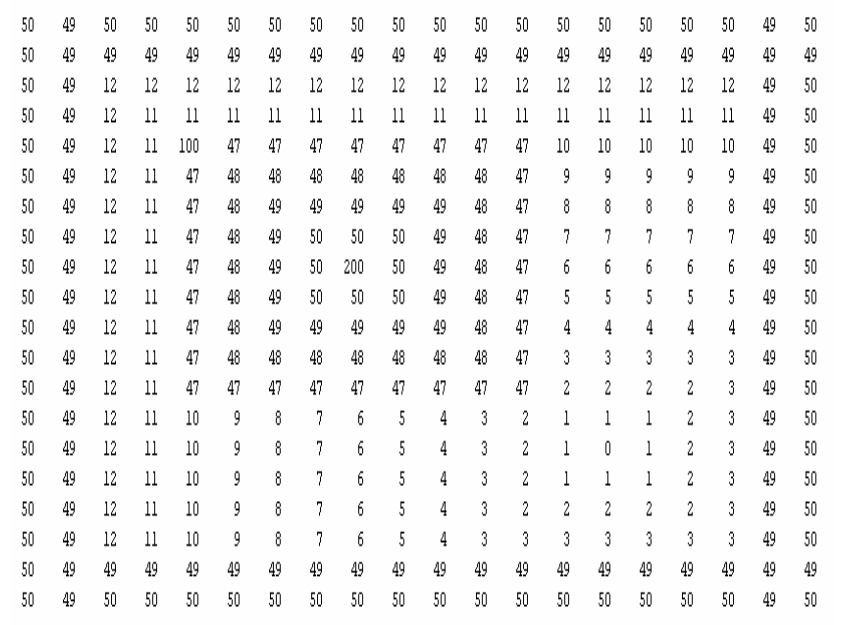
\includegraphics[width=5cm]{imag.png}
    \caption{Representación gráfica }
\end{figure}
De esa forma el robot se moverá de su posición a la que lo deje más cerca de objetivos y que al mismo tiempo tenga un potencial menor o igual al que tiene, y así sucesivamente. 

Finalmente, el camino óptimo es el siguiente:
\begin{figure}[H]
    \centering
    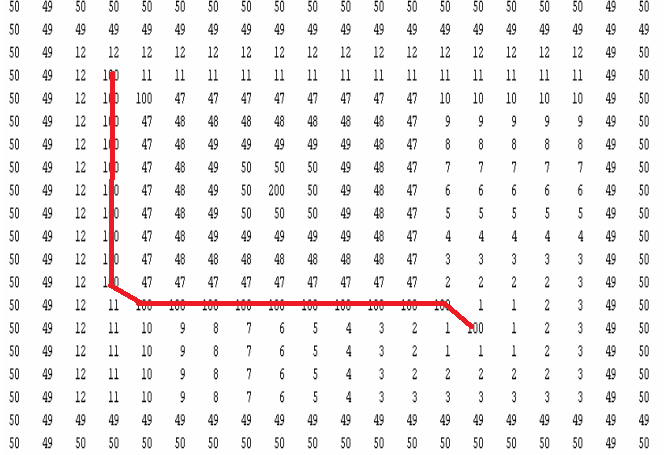
\includegraphics[width=5cm]{4.png}
    \caption{Ruta óptima}
    \label{sol1}
\end{figure}
El modelo presentado resulta ser un poco confuso y escaparse un poco del concepto de modelamiento matemático, es por esto que se llevo a cabo la elaboración del siguiente modelo de programación lineal.\\
\subsection{De forma general:}
Comenzamos creando una matriz de orden $NxN$ la cual representará el espacio donde se desplazará el robot, indicando el inicio de donde comienza su trayecto, los obstáculos y el final.\\
\begin{figure}[H]
 \[ \left( \begin{array}{ccc}
{x}_{11} & \cdots & {x}_{1n} \\
\vdots & \ddots & \vdots \\
{x}_{n1} & \cdots & {x}_{nn} \end{array} \right)\] 
\caption{Matriz general}
\end{figure}
Esta construcción tendrá las siguientes condiciones iniciales.
\begin{itemize}
    \item Se debe conocer las posiciones de los obstáculos.
    \item El final (meta) siempre será en ${x}_{nn}$.
    \item El comienzo será en ${x}_{11}$.
\end{itemize}
\textbf{Variables:}
\[
{x}_{ij}= \left\{ \begin{array}{lcc}
             1: &   robot\;pasa\;por\;ij \\
             \\ 0: &  robot\;no\;pasa\;por\;ij \\
             
             \end{array}
   \right.
\]
\textbf{Función Objetivo:}
\[ Min\;z = \sum_{i=1}^n\sum_{j=1}^n{x}_{ij}\]
\textbf{Restricciones}
\begin{itemize}
    \item Condiciones para obstáculos \\
    \begin{center}
        ${x}_{ij} = 0\;\;Para\;cada\;obstaculo$\\
        ${x}_{11} = 1\;\;Inicio$\\
        ${x}_{nn} = 1\;\;Final$\\
        ${x}_{12}+ {x}_{21} = 1 \cdot   Extras$\\
        ${x}_{n-1,n}+ {x}_{n,n-1} = 1 \cdot   Extras$\\ 
    \end{center}
    \item Condiciones para posición
    \begin{center}
        ${2x}_{ij} \leq{x}_{i-1,j}+{x}_{i+1,j}+{x}_{i,j-1}+{x}_{i,j+1}$\\
    \end{center}
\end{itemize}
\textbf{Dominio}
\begin{center}
        $0<i\leq n$\\
        $0<j\leq n$\\
        $\forall {x}_{ij} \in \{0,1\}$
    \end{center}
\subsection{Un caso en especifico}
En el presente documento resolveremos el problema de \textit{Robot Path Planning} para un caso en especifico que se describirá a continuación.\\

\begin{table}[H]
\centering
\begin{tabular}{lccccc}
                       & \multicolumn{1}{l}{1}  & \multicolumn{1}{l}{2}  & \multicolumn{1}{l}{3}  & \multicolumn{1}{l}{4}  & \multicolumn{1}{l}{5}         \\ \cline{2-6} 
\multicolumn{1}{l|}{1} & \multicolumn{1}{c|}{O} & \multicolumn{1}{c|}{}  & \multicolumn{1}{c|}{x} & \multicolumn{1}{c|}{x} & \multicolumn{1}{c|}{x}        \\ \cline{2-6} 
\multicolumn{1}{l|}{2} & \multicolumn{1}{c|}{}  & \multicolumn{1}{c|}{}  & \multicolumn{1}{c|}{}  & \multicolumn{1}{c|}{}  & \multicolumn{1}{c|}{}         \\ \cline{2-6} 
\multicolumn{1}{l|}{3} & \multicolumn{1}{c|}{x} & \multicolumn{1}{c|}{x} & \multicolumn{1}{c|}{}  & \multicolumn{1}{c|}{}  & \multicolumn{1}{c|}{}         \\ \cline{2-6} 
\multicolumn{1}{l|}{4} & \multicolumn{1}{c|}{x} & \multicolumn{1}{c|}{x} & \multicolumn{1}{c|}{x} & \multicolumn{1}{c|}{}  & \multicolumn{1}{c|}{}         \\ \cline{2-6} 
\multicolumn{1}{l|}{5} & \multicolumn{1}{c|}{x} & \multicolumn{1}{c|}{x} & \multicolumn{1}{c|}{x} & \multicolumn{1}{c|}{}  & \multicolumn{1}{c|}{$\Delta$} \\ \cline{2-6} 
\end{tabular}
\end{table}
Donde:\\
$O:\; Robot$\\
$\Delta:\;Meta$\\
$X:\;Obstaculos$\\
Además el robot solo se puede mover en dirección arriba, abajo, izquierda, derecha.\\

\textbf{Variables: }Descritas en el caso general.\\

\textbf{Función Objetivo}\\

\[ Min\;z = \sum_{i=1}^5\sum_{j=1}^5{x}_{ij}\] \\

\textbf{Restricciones}\\

\textbf{\textit{Obstáculos:} }
${x}_{31}={x}_{41}={x}_{51}={x}_{13}={x}_{23}={x}_{14}={x}_{24}={x}_{34}={x}_{15}={x}_{25}= {x}_{35}=0$\\

\textbf{\textit{Inicio: }}
\begin{center}
   ${x}_{11}=1$\\ 
\end{center}

\textbf{\textit{Final: }}
\begin{center}
    ${x}_{55}=1$\\
\end{center}


\textbf{\textit{Posición:} }\\
\begin{table}[H]
\centering
\begin{tabular}{lll}
${2x}_{12}\leq {x}_{11}+{x}_{22}$                   &  & ${x}_{11}+{x}_{22}\geq 1$                   \\
${2x}_{21}\leq {x}_{11}+{x}_{22}$                   &  & ${x}_{11}+{x}_{22}\geq 1$                   \\
${2x}_{22}\leq {x}_{12}+{x}_{21}+{x}_{32}$          &  & ${x}_{12}+{x}_{21}+{x}_{32}\geq 1$          \\
${2x}_{32}\leq {x}_{42}+{x}_{22}+{x}_{33}$          &  & ${x}_{42}+{x}_{22}+{x}_{33}\geq 1$          \\
${2x}_{42}\leq {x}_{52}+{x}_{43}+{x}_{32}$          &  & ${x}_{52}+{x}_{43}+{x}_{32}\geq 1$          \\
${2x}_{52}\leq {x}_{42}+{x}_{53}$                   &  & ${x}_{42}+{x}_{53}\geq 1$                   \\
${2x}_{33}\leq {x}_{32}+{x}_{43}$                   &  & ${x}_{32}+{x}_{43}\geq 1$                   \\
${2x}_{43}\leq {x}_{33}+{x}_{42}+{x}_{53}+{x}_{44}$ &  & ${x}_{33}+{x}_{42}+{x}_{53}+{x}_{44}\geq 1$ \\
${2x}_{53}\leq {x}_{52}+{x}_{43}+{x}_{54}$          &  & ${x}_{52}+{x}_{43}+{x}_{54}\geq 1$          \\
${2x}_{44}\leq {x}_{43}+{x}_{54}+{x}_{45}$          &  & ${x}_{43}+{x}_{54}+{x}_{45}\geq 1$          \\
${2x}_{54}\leq {x}_{53}+{x}_{55}++{x}_{44}$         &  & ${x}_{53}+{x}_{55}+{x}_{44}\geq 1$          \\
${2x}_{45}\leq {x}_{44}+{x}_{55}$                   &  & ${x}_{44}+{x}_{55}\geq 1$                  
\end{tabular}
\end{table}

\textbf{Extras}\\
\begin{center}
 ${x}_{54}+{x}_{45}=1$\\
 ${x}_{12}+{x}_{21}=1$\\
\end{center}
\section{Representación y Entorno de ejecución}
Debido a la dificultad presente en el modelo de método potencial y a las herramientas que se utilizan para llevar a cabo su implementación, se decidió elegir otro camino para resolver el presente problema de seleccionar la ruta óptima de un robot.\\
El modelo de programación lineal resultó ser el más practico debido a que existen herramientas digitales accesibles a todo público( como Lingo) que permiten resolver un modelo lineal con una entendible interpretación de la solución.\\
El modelo presentado en la sección anterior se desarrolló y ejecutó en el software \textit{Lingo} en su versión 17.0.79 (12 Junio 2018) para Mac64.\\
El ordenador que compiló dicho código corresponde a un Macbook Air 2017 con sistema operativo macOS Mojave.\\

\section{Resultados}
Según lo expuesto en la sección de entorno de ejecución, Lingo nos facilitó el desarrollo y solución del modelo planteado, entregando la información que se puede observar en la Figura \href{solucion-lingo} presente más adelante.
De esta figura se puede apreciar que las variables por la cual deberá pasar el robot corresponden a: ${x}_{11},\;{x}_{12},\;{x}_{22},\;{x}_{32},\;{x}_{33},\;{x}_{43},\;{x}_{53},\;{x}_{54},\;{x}_{55}\;$\\ 
Las cuales otorgan un valor a la función objetivo correspondiente a 9, que en este caso sería la mínima cantidad de movimientos que tiene que realizar el robot para llegar  su destino sin pasar por los obstáculos, considerando el inicio y el término.\\
\begin{figure}[H]
    \centering
    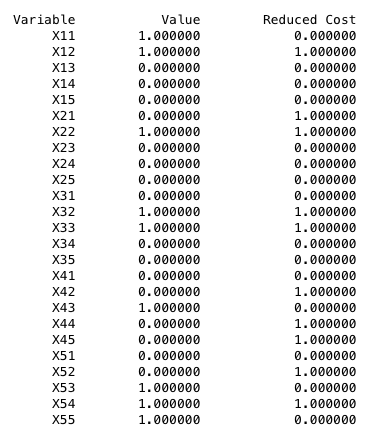
\includegraphics[width=6.5cm]{2.png}
    \caption{Solución entregada por Software:Lingo}
    \label{solucion-lingo}
\end{figure}

Dicha solución representada gráficamente en el mapa queda de la siguiente forma.
\begin{table}[H]
\centering
\begin{tabular}{llllll}
                       & 1                                                                     & 2                                             & 3                                             & 4                                             & 5                                                     \\ \cline{2-6} 
\multicolumn{1}{l|}{1} & \multicolumn{1}{l|}{\cellcolor[HTML]{32CB00}{\color[HTML]{000000} O}} & \multicolumn{1}{l|}{\cellcolor[HTML]{32CB00}} & \multicolumn{1}{l|}{x}                        & \multicolumn{1}{l|}{x}                        & \multicolumn{1}{l|}{x}                                \\ \cline{2-6} 
\multicolumn{1}{l|}{2} & \multicolumn{1}{l|}{}                                                 & \multicolumn{1}{l|}{\cellcolor[HTML]{32CB00}} & \multicolumn{1}{l|}{\cellcolor[HTML]{32CB00}} & \multicolumn{1}{l|}{}                         & \multicolumn{1}{l|}{}                                 \\ \cline{2-6} 
\multicolumn{1}{l|}{3} & \multicolumn{1}{l|}{x}                                                & \multicolumn{1}{l|}{x}                        & \multicolumn{1}{l|}{\cellcolor[HTML]{32CB00}} & \multicolumn{1}{l|}{\cellcolor[HTML]{32CB00}} & \multicolumn{1}{l|}{\cellcolor[HTML]{32CB00}}         \\ \cline{2-6} 
\multicolumn{1}{l|}{4} & \multicolumn{1}{l|}{x}                                                & \multicolumn{1}{l|}{x}                        & \multicolumn{1}{l|}{x}                        & \multicolumn{1}{l|}{}                         & \multicolumn{1}{l|}{\cellcolor[HTML]{32CB00}}         \\ \cline{2-6} 
\multicolumn{1}{l|}{5} & \multicolumn{1}{l|}{x}                                                & \multicolumn{1}{l|}{x}                        & \multicolumn{1}{l|}{x}                        & \multicolumn{1}{l|}{}                         & \multicolumn{1}{l|}{\cellcolor[HTML]{32CB00}$\Delta$} \\ \cline{2-6} 
\end{tabular}
\caption{Representación de camino óptimo}
\end{table}

\section{Benchmark o Comparación con resultados en Literatura}
El modelo presentado y analizado en el presente documento se basó indicando que el robot solo puede desplazarse horizontalmente y verticalmente, por lo cual un modelo que considere movimientos en diagonales, o no tan segmentados en casillas, pueden obtener un mejor óptimo. Lo anterior presentaba una dificultad mayor al momento de plantear nuestro modelo de programación lineal, el cual buscando en internet o similares resulta muy difícil de hallar, debido a que asume estos supuestos que encapsulan a una representación que en la vida real no será la más óptima, sin embargo, existen varías formas de enfrentarse al problema de \textit{Robot Path Planning} entre ellas y la que más se asemeja a los resultados presentados, es una solución con programación dinámica. Tal solución posee varios algoritmos sobre como encontrar un óptimo, entre ellos Bellman-Ford y Kwok-Driessen\cite{Dynamic:1957}.\\

Al observar este método de programación dinámica se encuentran similitudes, como por ejemplo, en el algoritmo de Kwok-Driessen se parte creando una matriz de NxN donde a cada elemento de la matriz se le asocia un estado del entorno según su  localización  dentro  del  mismo, correspondiente a 0 si el estado es prohibido o 1 si el estado es libre \cite{PlanificacionPD:2011}, cuya interpretación es similar a la presentada en el modelo de programación lineal elegido para solucionar el problema de \textit{Robot Path Planning} dispuesto en este escrito.\\

Otro método y tal como se señaló en secciones anteriores corresponde al método potencial, el cual puede resultar más preciso obteniendo trayectorias en tiempo real a partir del plano (campo de fuerza), ayudando al control y planificación de caminos, por ejemplo, útil cuando los obstáculos pueden estar en movimiento. Dicho modelo también detalla una matriz inicial, pero modificable con el tiempo, debido a que representa numéricamente el campo potencial desde el robot hacia el punto donde puede o no haber un obstáculo.\\

Sin embargo, el método tiene una gran desventaja, la aparición de mínimos locales, es decir, este método funciona dando al punto objetivo un valor ''0'', pero que ocurre cuando e el campo de fuerzas (plano donde el robot se mueve) existen otros puntos donde la fuerzas se anulen, pueden llevar al robot a confundirse y no llegar a el objetivo.\\

En cuanto a calidad de solución esta depende del algoritmo que se utilice para solucionar el problema de \textit{Robot Path Planning}, si se consideran diversos factores, entre otros. De los métodos analizados y vistos el más efectivo cuanto a solución óptima y que considera movimientos no solamente rectilíneo es el de programación lineal, utilizando el algoritmo de Bellman-Ford Optimizado \cite{PlanificacionPD:2011}.\\
Como un problema de programación dinámica que considera varios factores y movimientos genera más restricciones, en cuanto al tiempo de ejecución del modelo de programación lineal resulta más conveniente, con los supuestos descritos, se evitan gran porcentaje de iteraciones. 


\section{Conclusiones}

Como ya se ha mencionado antes Robot Path Planning Problem es NP-Completo, por lo que no existe manera óptima de resolverlo, aún así, se ha logrado identificar un método que consigue presentar un buen algoritmo para la resolución del problema, el método del campo potencial, permite identificar mediante cargas y polaridades el camino a seguir por el robot, si bien presenta grandes ventajas, como generar trayectorias continuas y en tiempo real, facilitando el control y la planificación de caminos, se presenta una gran desventaja, la aparición de mínimos locales, que podría impedir que el robot alcance su objetivo y existen puntos en los que se anulen las fuerzas.

Utilizar un buen método para la planificación de caminos del robot puede hacer que un robot se desplace de una mejor manera al reducir su camino recorrido, lo cual permite simular que el robot analiza los caminos y selecciona el mejor para desplazarse. Los constantes avances de investigación en inteligencia artificial podrían ayudar a resolver este tipo de problemas de manera más dinámica.

En base a esto, queda como trabajo futuro, mejorar el algoritmo, o identificar e implementar un algoritmo mediante el cual se asegure que de haber un camino el robot siempre sea capaz de llegar desde el punto inicial al punto final.


\bibliographystyle{plain}
\bibliography{bibliografia}

\end{document}
